\paragraph{Composition panels.}
Reference checks retain 31 of 78 metadata-eligible compositions, including 21 used in earlier development. We select 12 for source development and use the remaining 10 for the subsequent test. The latter contain 17--28 atoms and are absent from all 3,902,107 processed training and 39,415 validation rows, as checked by exact atom-count vectors. References determine eligibility only. Both panels use the same two fine-tuning runs; Section~\ref{sec:fresh-physics} describes the further 24-composition test.

\begin{table}[t]
\centering
\caption{Valid outputs over all attempts for source variants sharing a self-conditioned backbone and 128 sampling calls. The additional panel evaluates checkpoints fixed after development.}
\begin{tabular}{llrrr}
\toprule
Set & Run & Gaussian & Shell tree & Harmonic tree\\
\midrule
Development (12) & 1 &357/768&417/768&436/768\\
                 & 2 &377/768&342/768&388/768\\
Additional (10)  & 1 &326/640&---&413/640\\
                 & 2 &349/640&---&375/640\\
\bottomrule
\end{tabular}\label{tab:main}
\end{table}

On the development panel, harmonic improves graph validity over isotropic Gaussian by 5.86 points (paired 95\% CI [2.67,8.98]; composition interval [0.52,12.17]). Both runs improve, especially run 1. Harmonic also exceeds the shell-tree control by 4.23 points; shell minus harmonic has interval [-7.29,-1.11].

On the 10-composition test, graph validity rises from 52.73\% to 61.56\%, a gain of 8.83 points (paired CI [5.08,12.50]; composition interval [4.84,12.66]). Contact-geometric validity gains 9.69 points [6.33,12.89]. All graph-valid outputs have distinct connectivities within composition, and no validator errors occur. Sampling time for 640 outputs is nearly identical: harmonic/Gaussian take 175.73/175.43 seconds in run 1 and 178.20/177.74 in run 2.

\begin{figure}[t]
\centering
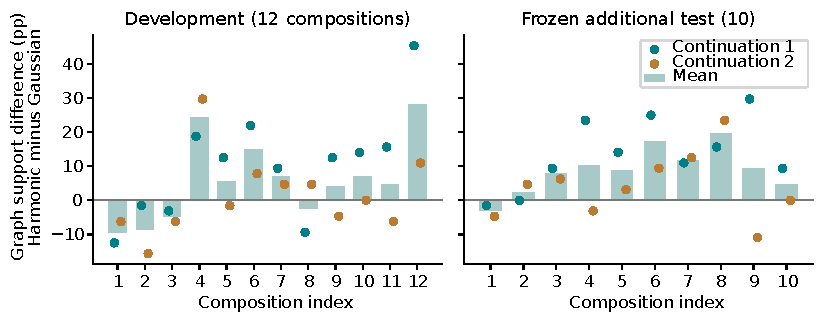
\includegraphics[width=\linewidth]{../research/figures/final_complete_v1/figures/composition_effects.pdf}
\caption{Per-composition harmonic-minus-Gaussian graph validity. Points show individual fine-tuning runs and bars their mean. Both panels use the same fitted models.}\label{fig:effects}
\end{figure}

\paragraph{Control for source covariance.}
To test whether the source benefit is explained by its covariance, we compare
against a single Gaussian with approximately the same covariance as the harmonic
mixture. We estimate that covariance from 128 trees and average over permutations
of identical atom species. An independent 8,192-tree estimate gives a relative
Frobenius error of 1.85--6.25\% across the 22 compositions. We match the training
data, optimizer, network, and sampling budgets. This follow-up compares the new
Gaussian models with the already frozen harmonic checkpoints.

\begin{table}[t]
\centering
\caption{Covariance-matched Gaussian versus harmonic source. Entries count
valid outputs over all attempts. Training and inference budgets are matched;
the Gaussian uses the calibrated covariance estimate from 128 trees.}
\begin{tabular}{llrr}
\toprule
Set & Run & Covariance Gaussian & Harmonic tree\\
\midrule
Development & 1 &332/768&436/768\\
            & 2 &313/768&388/768\\
Additional  & 1 &286/640&413/640\\
            & 2 &305/640&375/640\\
\bottomrule
\end{tabular}\label{tab:covariance}
\end{table}

Harmonic improves graph validity over this Gaussian by 11.65 percentage points
on development (paired 95\% interval [8.59,14.78]; descriptive composition interval
[8.07,15.43]) and 15.39 points on the additional set (paired [11.64,19.06];
composition [11.95,18.98]). The difference is positive in both runs on both sets.
The covariance-matched Gaussian also performs worse than the isotropic Gaussian.
These results support a benefit beyond this calibrated second-moment approximation,
consistent with a contribution from the mixture structure. The comparison adds
2,816 outputs while holding parameter count, initial self-conditioning weights,
training structures, and optimization fixed.

